\documentclass[a4paper]{article}
\usepackage{amsmath}
\usepackage{bm}
\usepackage{graphicx}
\graphicspath{{images/}}
\usepackage{pgfplots}
\usepackage{siunitx}
\usepackage{tikz}
\usepackage{xspace}

\newcommand{\MATLAB}{\textsc{Matlab}\xspace}

\title{Optical Fibres and Optocommunication --- Exam questions}
\author{Sergiusz Warga}

\begin{document}

\maketitle
\tableofcontents

\section{TM wave}
Question: Draw the plot showing dependence of $r_H$ and $\phi_H$ upon incidence angle for TM wave. Explain the origin and the meaning of characteristic points on this plot. Indicate orientation of the $E$ and $H$ vectors with respect to incidence plane.\bigskip

\section{TE wave}
Question: Draw the plot showing dependence of $r_E$ and $\phi_E$ upon incidence angle for TE wave. Explain the origin and the meaning of characteristic points on this plot. Indicate orientation of the $E$ and $H$ vectors with respect to incidence plane.\bigskip

%% https://sci-hub.do/https://www.osapublishing.org/josaa/viewmedia.cfm?uri=josaa-21-8-1559&seq=0

\nocite{optics}

Light can be modelled as the electromagnetic disturbances -- a wave -- propagating through the electromagnetic field. In optocommunication we use a plane wave solution to the Maxwell's equations, which describes the changes of electric $\vec{E}$ and magnetic $\vec {B}$ fields, presented in Figure~\ref{fig:plane-wave}. We call such a wave a transverse electric and magnetic field (TEM) wave. 
\begin{figure}[h]
    \centering
    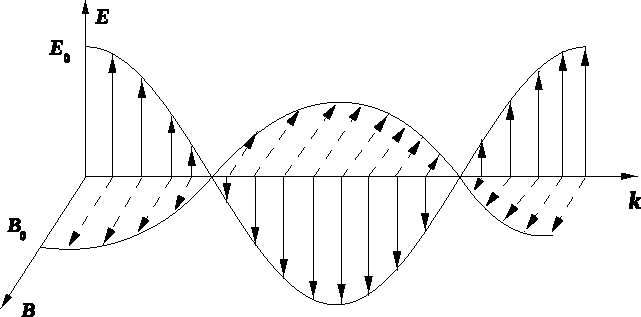
\includegraphics[width=0.7\textwidth]{images/TM_wave_plane_wave.pdf}
    \caption{A homogeneous plane wave; electric and magnetic fields are transverse to the direction of propagation and also to each other. From~\cite{optics}}
    \label{fig:plane-wave}
\end{figure}

We may also distinguish the TE and TH modes -- in the TE mode $\vec{E}$ changes are orthogonal to the incidence plane. In a three-dimensional Cartesian coordinate system with basis $B = \{\bm{\hat{n}}, \bm{\hat{\pi}}, \bm{\hat{\sigma}}\}$ and propagation direction $\bm{k}$ as presented in Figure~\ref{fig:boundary}, electric field variations would be observed only in $\bm{\sigma}$ axis, thus:
\begin{align*}
    \vec{E} &= [0, E_y, 0] & \vec{H} &= [H_x, 0, H_z]
\end{align*}
\begin{figure}[ht]
    \centering
    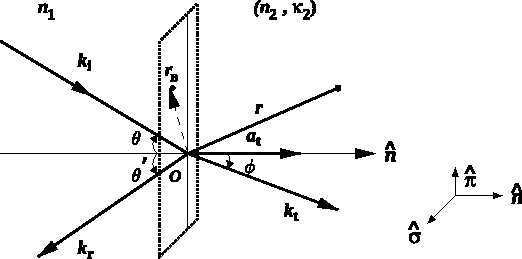
\includegraphics{images/reflection_at_boundary.pdf}
    \caption{Reflection and transmission of a wave at a plane boundary. From~\cite{optics}}
    \label{fig:boundary}
\end{figure}
Based on~\cite[ch.~1.7]{optics} and~\cite{Urbanczyk} we may denote a reflection coefficient for the orthogonally polarized wave $r_\sigma$  as
\begin{equation}
    r_{\sigma ext} = \frac{n_1\cos{\theta} - n_2\cos{\phi}}{n_1\cos{\theta} + n_2\cos{\phi}},
\end{equation}
where the refraction angle $\phi$ is
\begin{equation}
    \phi = \arcsin{\frac{n_1\sin{\theta}}{n_2}}
\end{equation}
for the external reflections (when $\theta < \theta_c$) and
\begin{equation}
    \label{eq:r-sig-int}
    r_{\sigma int} = \frac{n_1\cos{\theta} - i\sqrt{n_1^2\sin^2{\theta} - n_2^2}}{n_1\cos{\theta} + i\sqrt{n_1^2\sin^2{\theta} - n_2^2}} = e^{-i2\phi_0},
\end{equation}
where the phase change $2\phi_0$ is
\begin{equation}
    \phi_0 = \arctan{\frac{\sqrt{n_1^2\sin^2{\theta} - n_2^2}}{n_1\cos{\theta}}}.
\end{equation}
for the internal reflections (when $\theta > \theta_c$). 

As we may see in Equation~\ref{eq:r-sig-int} the reflection coefficient has unit magnitude for any angle exceeding the critical angle, thus the reflection is total.  $r_{\sigma int}$ being complex implies that the reflected field will not be in phase with the incident one and its phase change will grow from $2\phi_0=0$ at $\theta = \theta_c$ to $2\phi_0=\pi$ at $\theta = \frac{\pi}{2}$.

\begin{figure}[h]
    \centering
    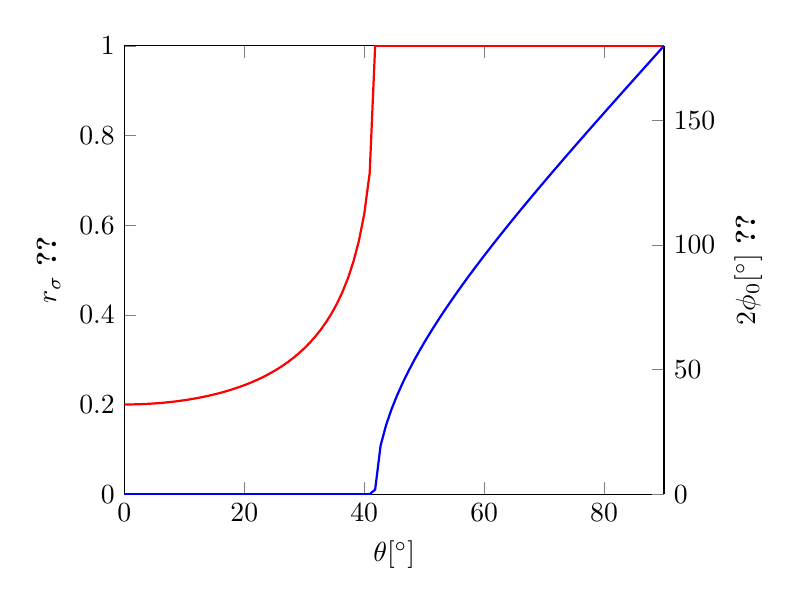
\begin{tikzpicture}
        \begin{axis}[
            axis y line* = left,
            xmin = 0, xmax= 90,
            ymin = 0, ymax = 1,
            xlabel = {$\theta [\si{\degree}]$},
            ylabel = {$r_\sigma$ \ref{plot:r}},
        ]
        \addplot[
            color=red,
            thick,
        ] table[row sep=crcr] {
            0	0.2\\
            0.909090909090909	0.200075548358143\\
            1.81818181818182	0.200302474323788\\
            2.72727272727273	0.200681623239942\\
            3.63636363636364	0.20121441295981\\
            4.54545454545455	0.20190284744675\\
            5.45454545454545	0.202749536175467\\
            6.36363636363636	0.20375771970972\\
            7.27272727272727	0.204931301959892\\
            8.18181818181818	0.206274889768904\\
            9.09090909090909	0.207793840642697\\
            10	0.20949431963852\\
            10.9090909090909	0.211383366659131\\
            11.8181818181818	0.21346897568415\\
            12.7272727272727	0.215760187815008\\
            13.6363636363636	0.218267200434693\\
            14.5454545454545	0.221001495310923\\
            15.4545454545455	0.223975989131789\\
            16.3636363636364	0.227205210796962\\
            17.2727272727273	0.230705510849594\\
            18.1818181818182	0.234495309798338\\
            19.0909090909091	0.238595393847125\\
            20	0.243029268863856\\
            20.9090909090909	0.247823586476549\\
            21.8181818181818	0.253008660269373\\
            22.7272727272727	0.25861909556895\\
            23.6363636363636	0.264694563859932\\
            24.5454545454545	0.271280763335456\\
            25.4545454545455	0.27843062181496\\
            26.3636363636364	0.286205819319164\\
            27.2727272727273	0.294678738238488\\
            28.1818181818182	0.303934994516478\\
            29.0909090909091	0.31407677226833\\
            30	0.325227291513248\\
            30.9090909090909	0.337536910103694\\
            31.8181818181818	0.351191643599362\\
            32.7272727272727	0.366425370146303\\
            33.6363636363636	0.383537849309218\\
            34.5454545454545	0.402922298925275\\
            35.4545454545455	0.425109485950506\\
            36.3636363636364	0.450842156114725\\
            37.2727272727273	0.481209720776053\\
            38.1818181818182	0.517915584981499\\
            39.0909090909091	0.563881382374634\\
            40	0.624914480999515\\
            40.9090909090909	0.716331282587392\\
            41.8181818181818	1\\
            42.7272727272727	1\\
            43.6363636363636	1\\
            44.5454545454545	1\\
            45.4545454545455	1\\
            46.3636363636364	1\\
            47.2727272727273	1\\
            48.1818181818182	1\\
            49.0909090909091	1\\
            50	1\\
            50.9090909090909	1\\
            51.8181818181818	1\\
            52.7272727272727	1\\
            53.6363636363636	1\\
            54.5454545454545	1\\
            55.4545454545455	1\\
            56.3636363636364	1\\
            57.2727272727273	1\\
            58.1818181818182	1\\
            59.0909090909091	1\\
            60	1\\
            60.9090909090909	1\\
            61.8181818181818	1\\
            62.7272727272727	1\\
            63.6363636363636	1\\
            64.5454545454545	1\\
            65.4545454545455	1\\
            66.3636363636364	1\\
            67.2727272727273	1\\
            68.1818181818182	1\\
            69.0909090909091	1\\
            70	1\\
            70.9090909090909	1\\
            71.8181818181818	1\\
            72.7272727272727	1\\
            73.6363636363636	1\\
            74.5454545454545	1\\
            75.4545454545455	1\\
            76.3636363636364	1\\
            77.2727272727273	1\\
            78.1818181818182	1\\
            79.0909090909091	1\\
            80	1\\
            80.9090909090909	1\\
            81.8181818181818	1\\
            82.7272727272727	1\\
            83.6363636363636	1\\
            84.5454545454545	1\\
            85.4545454545455	1\\
            86.3636363636364	1\\
            87.2727272727273	1\\
            88.1818181818182	1\\
            89.0909090909091	1\\
            90	1\\
            };\label{plot:r}
        \end{axis}
        \begin{axis}[
            axis y line* = right,
            axis x line = none,
            xmin = 0, xmax= 90,
            ymin = 0, ymax = 180,
            ylabel = {$2\phi_0[\si{\degree}]$ \ref{plot:phi}},
        ]
        \addplot[
            color=blue,
            thick,
        ] table[row sep=crcr] {
0	0\\
0.909090909090909	0\\
1.81818181818182	0\\
2.72727272727273	0\\
3.63636363636364	0\\
4.54545454545455	0\\
5.45454545454545	0\\
6.36363636363636	0\\
7.27272727272727	0\\
8.18181818181818	0\\
9.09090909090909	0\\
10	0\\
10.9090909090909	0\\
11.8181818181818	0\\
12.7272727272727	0\\
13.6363636363636	0\\
14.5454545454545	0\\
15.4545454545455	0\\
16.3636363636364	0\\
17.2727272727273	0\\
18.1818181818182	0\\
19.0909090909091	0\\
20	0\\
20.9090909090909	0\\
21.8181818181818	0\\
22.7272727272727	0\\
23.6363636363636	0\\
24.5454545454545	0\\
25.4545454545455	0\\
26.3636363636364	0\\
27.2727272727273	0\\
28.1818181818182	0\\
29.0909090909091	0\\
30	0\\
30.9090909090909	0\\
31.8181818181818	0\\
32.7272727272727	0\\
33.6363636363636	0\\
34.5454545454545	0\\
35.4545454545455	0\\
36.3636363636364	0\\
37.2727272727273	0\\
38.1818181818182	0\\
39.0909090909091	0\\
40	0\\
40.9090909090909	0\\
41.8181818181818	1.79598353355014\\
42.7272727272727	19.4985527790721\\
43.6363636363636	27.6686978780157\\
44.5454545454545	34.0490313573982\\
45.4545454545455	39.5165098076433\\
46.3636363636364	44.4098364890434\\
47.2727272727273	48.9019135841755\\
48.1818181818182	53.0949117606083\\
49.0909090909091	57.0550291633055\\
50	60.827982315635\\
50.9090909090909	64.4468620944837\\
51.8181818181818	67.9365018645714\\
52.7272727272727	71.3160805468255\\
53.6363636363636	74.6007602857732\\
54.5454545454545	77.8027627548109\\
55.4545454545455	80.9321024404152\\
56.3636363636364	83.9971015358059\\
57.2727272727273	87.0047608978192\\
58.1818181818182	89.9610332914974\\
59.0909090909091	92.871028584335\\
60	95.7391704772668\\
60.9090909090909	98.5693180354601\\
61.8181818181818	101.364861201285\\
62.7272727272727	104.128796773537\\
63.6363636363636	106.86378951345\\
64.5454545454545	109.572221781262\\
65.4545454545455	112.25623422553\\
66.3636363636364	114.917759418943\\
67.2727272727273	117.55854987984\\
68.1818181818182	120.180201585379\\
69.0909090909091	122.784173834979\\
70	125.371806137018\\
70.9090909090909	127.944332650903\\
71.8181818181818	130.502894608788\\
72.7272727272727	133.048551057815\\
73.6363636363636	135.582288198766\\
74.5454545454545	138.105027545984\\
75.4545454545455	140.617633092989\\
76.3636363636364	143.120917636091\\
77.2727272727273	145.615648382451\\
78.1818181818182	148.102551948301\\
79.0909090909091	150.582318836149\\
80	153.055607466088\\
80.9090909090909	155.523047825116\\
81.8181818181818	157.985244789165\\
82.7272727272727	160.442781164964\\
83.6363636363636	162.896220492662\\
84.5454545454545	165.346109644938\\
85.4545454545455	167.792981254162\\
86.3636363636364	170.237355995653\\
87.2727272727273	172.679744752279\\
88.1818181818182	175.120650683363\\
89.0909090909091	177.560571219063\\
90	180\\
        };\label{plot:phi}
        \end{axis}
    \end{tikzpicture}
    \caption{Variation of reflection coefficient $r_E$ and phase change $2\phi_0$ for $\frac{n_1}{n_2}=1.5$ computed in \MATLAB}
\end{figure}


\begin{enumerate}
    \item Define the loss coefficient for optical waveguides. In what units we measured losses in optical fibers.  
\end{enumerate}

\section{Numerical Aperture}\nocite{Swirniak, Sobon, Urbanczyk, optfib}

Question: Explain what is the numerical aperture of optical waveguide. How this parameter can be calculated for specific waveguide?\bigskip

Numerical aperture (NA) is an inherent parameter of all of the optical devices. It describes the maximum angle at which the indecent light might be accepted and thus propagated further. In case of an optical fibre it is directly related with the total internal reflection phenomenon, presented in Fig.\ref{fig:of_angles}, in which light beam hitting a core-cladding boundary at an angle greater than a critical angle $\theta_c$, will be reflected and propagated further.
\begin{figure}[h]
    \centering
    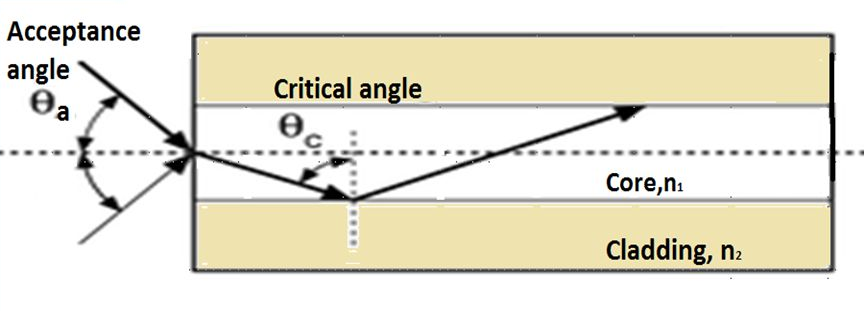
\includegraphics[width=0.7\textwidth]{Acceptance_Angle.png}
    \caption{Critical angle $\theta_c$ as measured between indecent ray and fibre transverse axis, and acceptance angle $\theta_a$ as measured between indecent ray and fibre longitudinal axis. $\theta_a$ depends only on the core and cladding refractive indices ($n_1$ and $n_2$). Based on~\cite{Sobon}}
    \label{fig:of_angles}
\end{figure}

All of the accepted and propagated light rays form an acceptance cone. Numerical aperture is then defined as
\begin{equation}
    NA = n\sin{\theta_a},
\end{equation}
where $n$ is a refractive index of a medium from which the ray hits the fibre's face\footnote{$\approx1$ for air.}. In practice, a different formula is used to calculate the optical fibre NA, incorporating its (core and cladding) refractive indices. The derivation of such a formula for a step-index fibre may be obtained straight from a Snell's law:
\begin{equation}
    \label{eqn:snell_law}
    n_1 \sin{\theta_1} = n_2 \sin{\theta_2}
\end{equation}

By increasing $\theta_1$ so that $\theta_2 = \frac{\pi}{4}$, and substituting $n_1$ and $n_2$ for the $n_{core}$ and $n_{clad}$ respectively, we obtain a critical angle formula:

\begin{equation}
    \theta_c = \arcsin{\frac{n_{clad}}{n_{core}}}
\end{equation}

Then, a relation between $\theta_a$ and $\theta_c$ may be represented as:

\begin{equation*}
    n\sin{\theta_a} = n_{core}\sin{\left(\frac{\pi}{4} - \theta_c\right)}
\end{equation*}

which can be transformed into

\begin{equation*}
\begin{split}
    n^2\sin^2{\theta_a} &= n^2_{core}\cos^2{\theta_c} \\
    n^2\sin^2{\theta_a} &= n^2_{core}\left(1 - \sin^2{\theta_c}\right) \\
    n^2\sin^2{\theta_a} &= n^2_{core} - n^2_{clad}
\end{split}
\end{equation*}

and finally:

\begin{equation}
    NA = n\sin{\theta_a} = \sqrt{n^2_{core} - n^2_{clad}}.
\end{equation}


5.	Write the characteristic equation for TE and  TM in planar waveguide. Plot the distribution of amplitude across the waveguide  in the mode TE2  (or other !).

6.	Define the cut-off wavelength for single mode fiber. Where most of energy of the mode close to cut-off is confined. What is the propagation constant of such mode. 

7.	Define the normalized propagation constant b. In what range this parameter can vary? 

8.	Write the unified characteristics equation for step-index fiber. Define all variables and explain for what purpose this equation is  used. 

9.	Define phase and group refractive indices, phase and group velocity of  EM wave. Explain the meaning of these parameters. 

10.	Plot the distribution of electric filed in the mode LP 2 1 yo  (or other !)

\section{Some task}
Question: Light of wavelength of 500nm has been introduced to the step-index optical fiber with a core diameter $2a=5\mu m$, $n_1=1.461$, $n_2=1.455$. Explain if this is a single mode fiber. What is the cut-off wavelength for this fiber?\bigskip

To determine the operation mode of such a fibre we may use a normalized frequency formula:
\begin{equation}\label{eq:norm-freq}
    V = \frac{2\pi a}{\lambda}\sqrt{n_{core}^2-n_{clad}^2} = 4.156
\end{equation}

The condition for the single-mode operation is $V<2.405$, therefore for $\lambda=500nm$ the considered fibre is multi-mode. To determine fibre's cutoff wavelength we simply transform Equation~\ref{eq:norm-freq} to obtain:
\begin{equation}
    \lambda_{cutoff} = \frac{2\pi a}{2.405}\sqrt{n_{core}^2-n_{clad}^2} = 864nm,
\end{equation}
above for which the fibre will be single-mode.


\section{Losses in silica fibers}
Question: Elaborate on the reasons for losses in silica fibres. Plot typical spectral characteristic of power loss in silica fibers, indicate the transmission windows.\bigskip

Fibre power loss describes the proportion of beam power leaving the fibre to the power of introduced light beam. It is usually represented by a fiber attenuation coefficient:
\begin{equation}
    \alpha = \frac{10}{L}\log_{10}\left(\frac{P_{out}}{P_{in}}\right) \left[\frac{dB}{km}\right]
\end{equation}
where $L$ is the fibre's length. With its use the efficient power on a given length could be calculated as:
\begin{equation}
    P(L) = P(0)e^{-\alpha L}
\end{equation}

\begin{figure}[h]
    \centering
    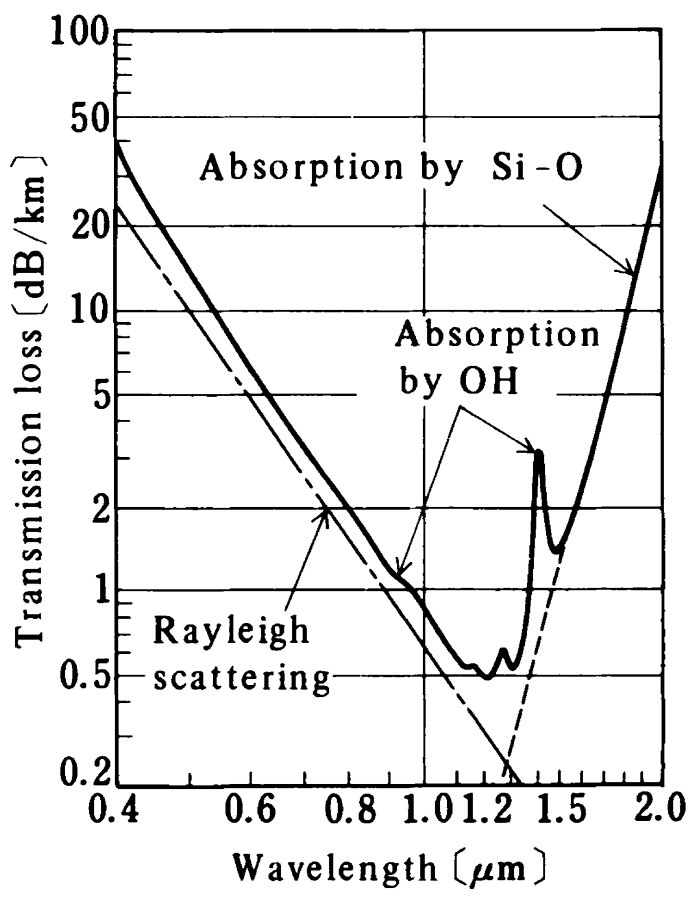
\includegraphics[width=0.5\textwidth]{images/losses.png}
    \caption{An example of the transmission-loss characteristics of low-loss optical fibres. Telecommunication windows visible here are $0.8\mu m$, $1.3\mu m$ and $1.55\mu m$. From~\cite{optfib}}
    \label{fig:my_label}
\end{figure}

Sources of these losses are manifold, but I will divide them here into three groups: (1) physical phenomena inherent to the silica, (2) impurities, (3) structural imperfections, both of internal and external origin.

\subsection{Inherent physical phenomena}

In the range from near ultra-violet to the far infra-red there are three main phenomena inducing power losses in the fibre: Rayleigh scattering, UV absorption and IR absorption.

The main cause of power losses in the visible spectrum is the Rayleigh scattering occurring due to the fluctuations of the refractive index\footnote{Of the order of $10^{-8}$.} throughout the core. These are introduced to the fibre in the manufacturing process during the glass solidification. Particles (atoms or molecules) several times smaller than the propagated wavelength can absorb the photon and re-radiate it in almost any direction. Rayleigh scattering increases towards the ultraviolet spectrum at $\approx\frac{1}{\lambda^4}$.

Photons of a sufficiently high energy, namely those of UV region, could be absorbed by the valence band electrons and excite them to the conductance band\footnote{Later this electron will emit a photon being a part of the scattered signal.}. 

In the infrared range the low-enegry photos are absorbed by the Si--O molecules and transformed into heat.

\subsection{Impurities}

Water and transition metal molecules are two important impurities introducing losses to the fibre. Hydroxyl OH group has a fundamental molecular vibration of $\lambda=2.8\mu m$ with second and third harmonics at 1.38 and 0.95$\mu m$. To suppress the second harmonic absorption below the SiO one, the water molecules cannot exceed 0.01 ppm.

In the past Cr, Mn, Co, Fe, Ni, Cu and V absorption was intensively observed, but today's good manufacturing process allows to ignore them.

\subsection{Structural imperfection}
Those may be constituted with the mechanical manipulation of the fibre such as bending, introducing geometrical  non-uniformity at the core-cladding boundary or with the imperfections at the connections (misalignment) and during the splicing.


13.	Draw a plot showing dependence of chromatic dispersion upon wavelength in different types of single mode fibers. Elaborate on the origin of chromatic dispersion in optical fibers.  

14.	Describe the origin of modal dispersion and the impact of mode mixing on  its behavior.

15.	Explain how birefringence can be induced in optical fibers. What is the highly birefringent fiber? 

\bibliographystyle{alpha}
\bibliography{bibliography}

\end{document}
